\documentclass{beamer}
\usetheme[pageofpages=de,% String used between the current page and the
                         % total page count
          bullet=circle,% Use circles instead of squares for bullets
          titleline=true,% Show a line below the frame title
          alternativetitlepage=true,% Use the fancy title page
          titlepagelogo=images/unlp,% Logo for the first page
          watermark={}, %info-watermark,% Watermark used in every page
          watermarkheight=12px,% Height of the watermark
          watermarkheightmult=4,% The watermark image is 4 times bigger
                                % than watermarkheight
          ]{Torino}

\usepackage{pgf}
% Basado en: http://www.tjansson.dk/?p=82

\usepackage[utf8x]{inputenc}
\setbeamercovered{transparent}

\usepackage{listings}
\usepackage{upquote}
\usepackage{xcolor}
\usepackage{array}
\lstset {
    basicstyle=\tiny, showstringspaces=no, frame=single,
    % Listings en español y con comillas simples copiables
    extendedchars=\true,
    inputencoding=utf8x,
    upquote=true,
    literate={á}{{\'a}}1
    {é}{{\'e}}1
    {í}{{\'i}}1
    {ó}{{\'o}}1
    {ú}{{\'u}}1
    {ñ}{{\~n}}1,
    language=C,
    upquote=true,
    breaklines=true
}

\hypersetup{%
    colorlinks=true,
    urlcolor=blue,
    linkcolor=blue,
    citecolor=blue,
}

% Para que funcione la inclusión de hyperref con utf8x
\PrerenderUnicode{á}
\PrerenderUnicode{é}
\PrerenderUnicode{í}
\PrerenderUnicode{ó}
\PrerenderUnicode{ú}


\title{XRemoteBot}
\subtitle{Un servicio para programar robots en forma remota}
\author{Fernando López}
\institute{Facultad de Informática \\ Universidad Nacional de La Plata}
\date{\the\year}

\newcommand{\proyecto}{``Programando con robots y software libre''}
\newcommand{\ipre}{``Institute for Personal Robots in Education''}

%\setbeamercolor{background canvas}{bg=}%transparent canvas
%\usepackage[firstpage]{draftwatermark}
%\SetWatermarkText{
\includegraphics{images/watermark}}
%\SetWatermarkAngle{0}
%\SetWatermarkLightness{0.8}
%\SetWatermarkScale{5}
%\SetWatermarkColor[rgb]{0.97,0.97,0.97}

\begin{document}

\frame{\titlepage \vspace{-0.5cm}
\vspace{0.5cm}
\hfill
\includegraphics[width=0.1\linewidth]{images/cc-by}
}

\frame{%
    \frametitle{Indice}
    \tableofcontents
}

\section{Introducción}

\subsection{Producto de la tesina}
\begin{frame}{Producto de la tesina}
    \begin{minipage}{0.5\linewidth}
        \begin{itemize}
            \item XRemoteBot
            \item Robots reales de forma remota
            \item Programación
        \end{itemize}
    \end{minipage}%
    \begin{minipage}{0.5\linewidth}
        \begin{figure}
            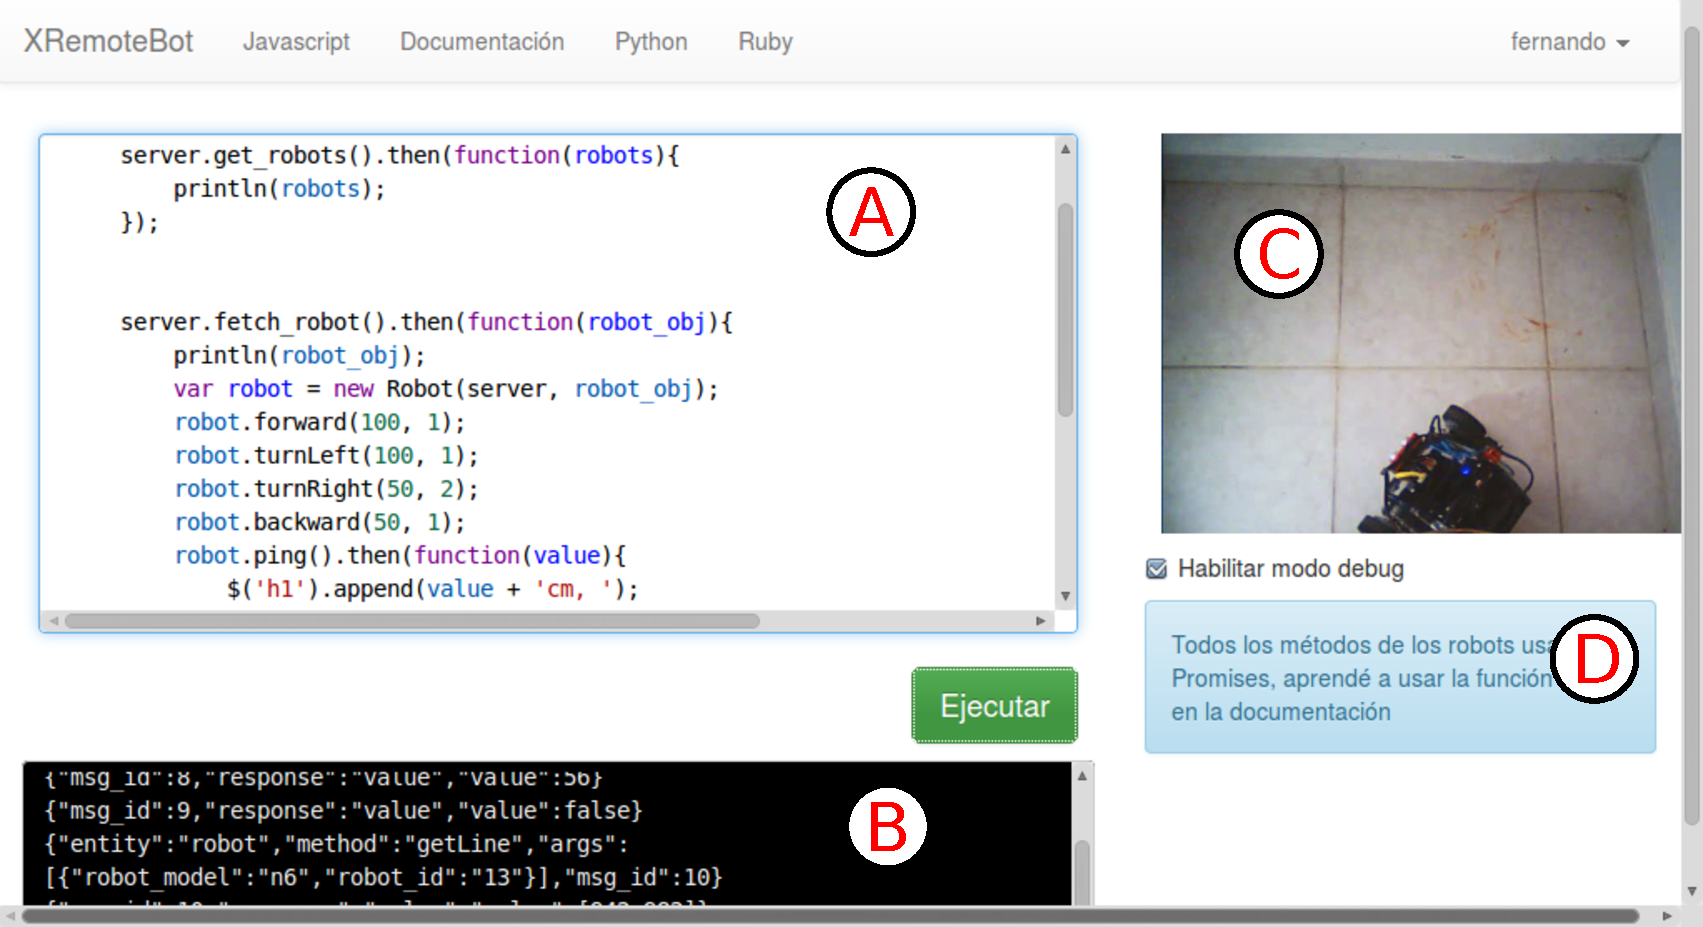
\includegraphics[width=\linewidth]{images/xremotebot_gui}
        \end{figure}
        \begin{figure}
            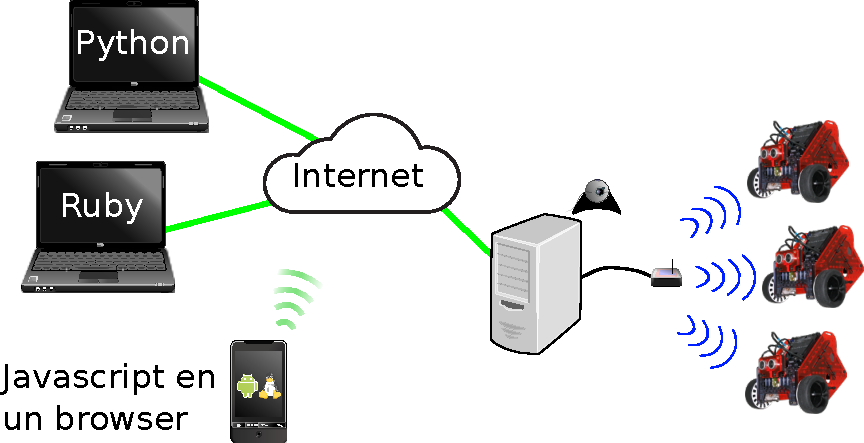
\includegraphics[width=\linewidth]{images/arquitectura_propuesta_wan}
        \end{figure}
    \end{minipage}
\end{frame}


\subsection{Motivación}
\begin{frame}{Motivación}{Proyecto}
    \begin{itemize}[<+->]
        \item Desde el año 2009 proyecto \proyecto{}
        \item Parallax Scribbler (2009)
        \item Multiplo N6 de RobotGroup (2011)
        \item Proyecto con YPF y Dirección de Escuelas Técnicas
            de la Provincia de Buenos Aires
    \end{itemize}
\end{frame}

\begin{frame}{Motivación}{Scribblers}
    \begin{minipage}[t]{0.7\linewidth}
        \begin{itemize}[<+->]
            \item Origen
            \item Biblioteca Myro
            \item Fluke
            \item Sensores
            \item Cómo los usamos
            \item Problemas:
                \begin{itemize}
                    \item Reconexión
                    \item Pilas
                    \item Compra
                \end{itemize}
        \end{itemize}
    \end{minipage}%
    \begin{minipage}[t]{0.3\linewidth}
        \begin{figure}
            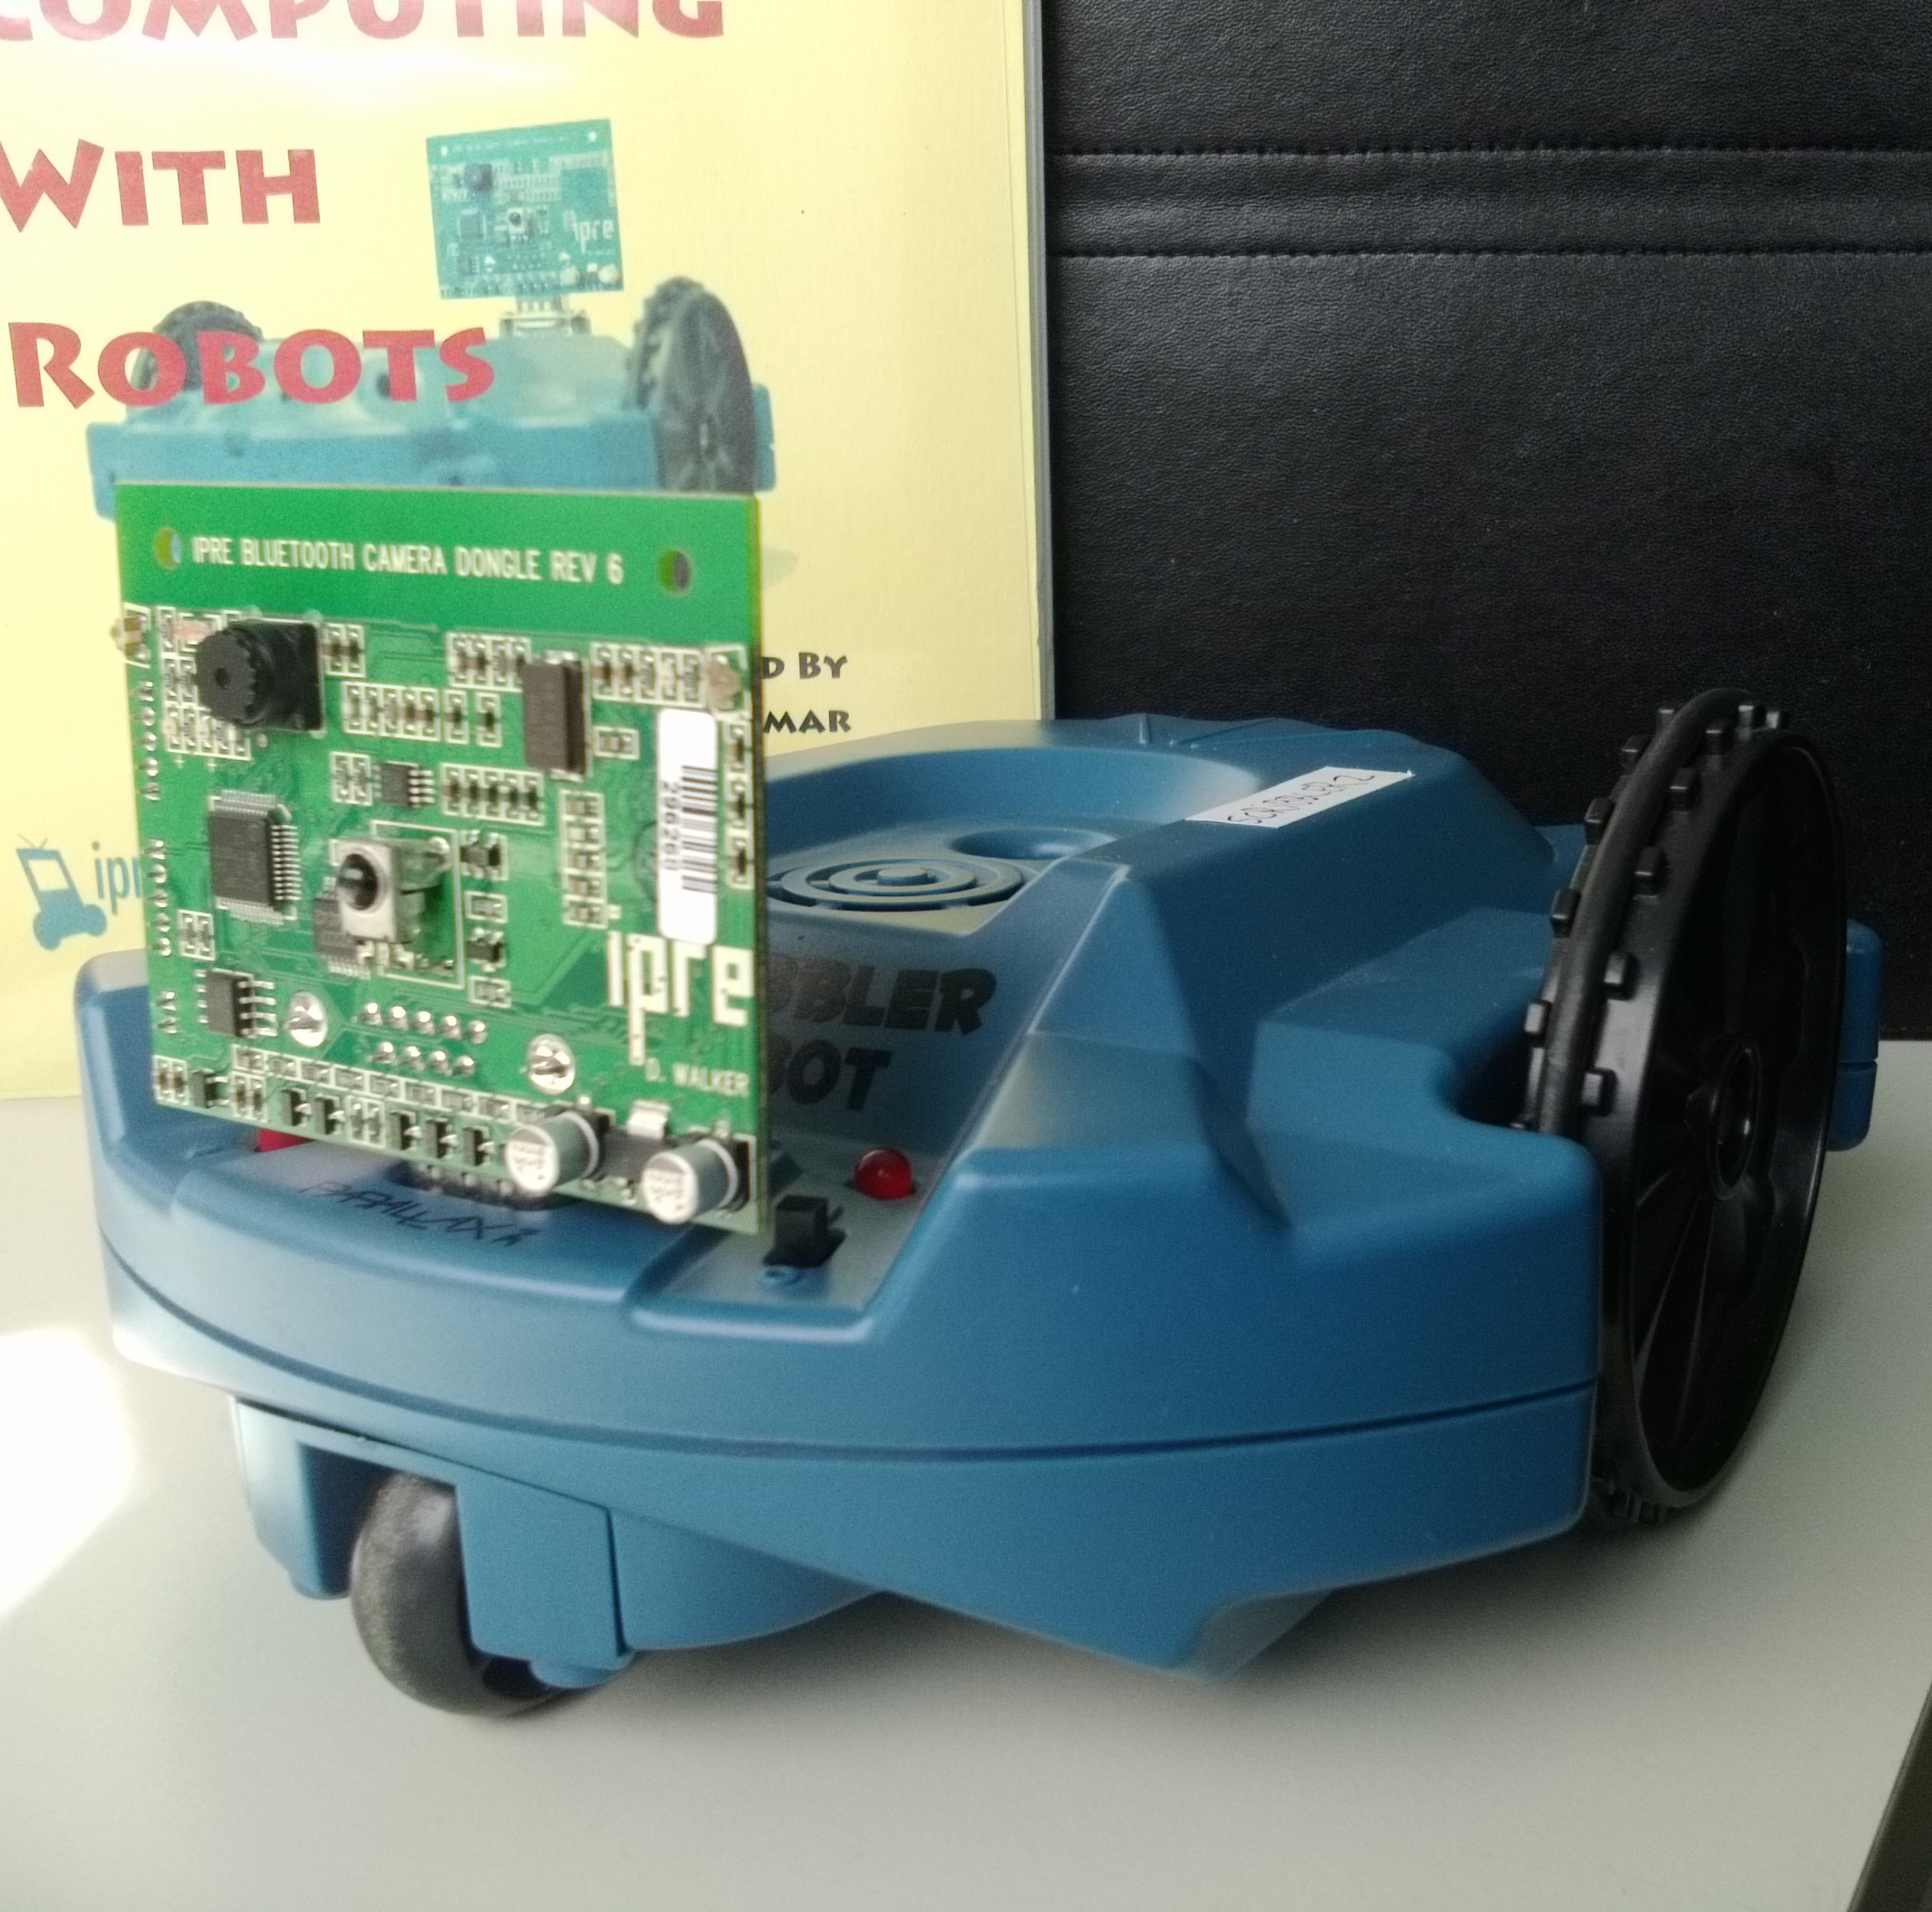
\includegraphics[width=\linewidth]{images/scribbler}
        \end{figure}
        \begin{figure}
            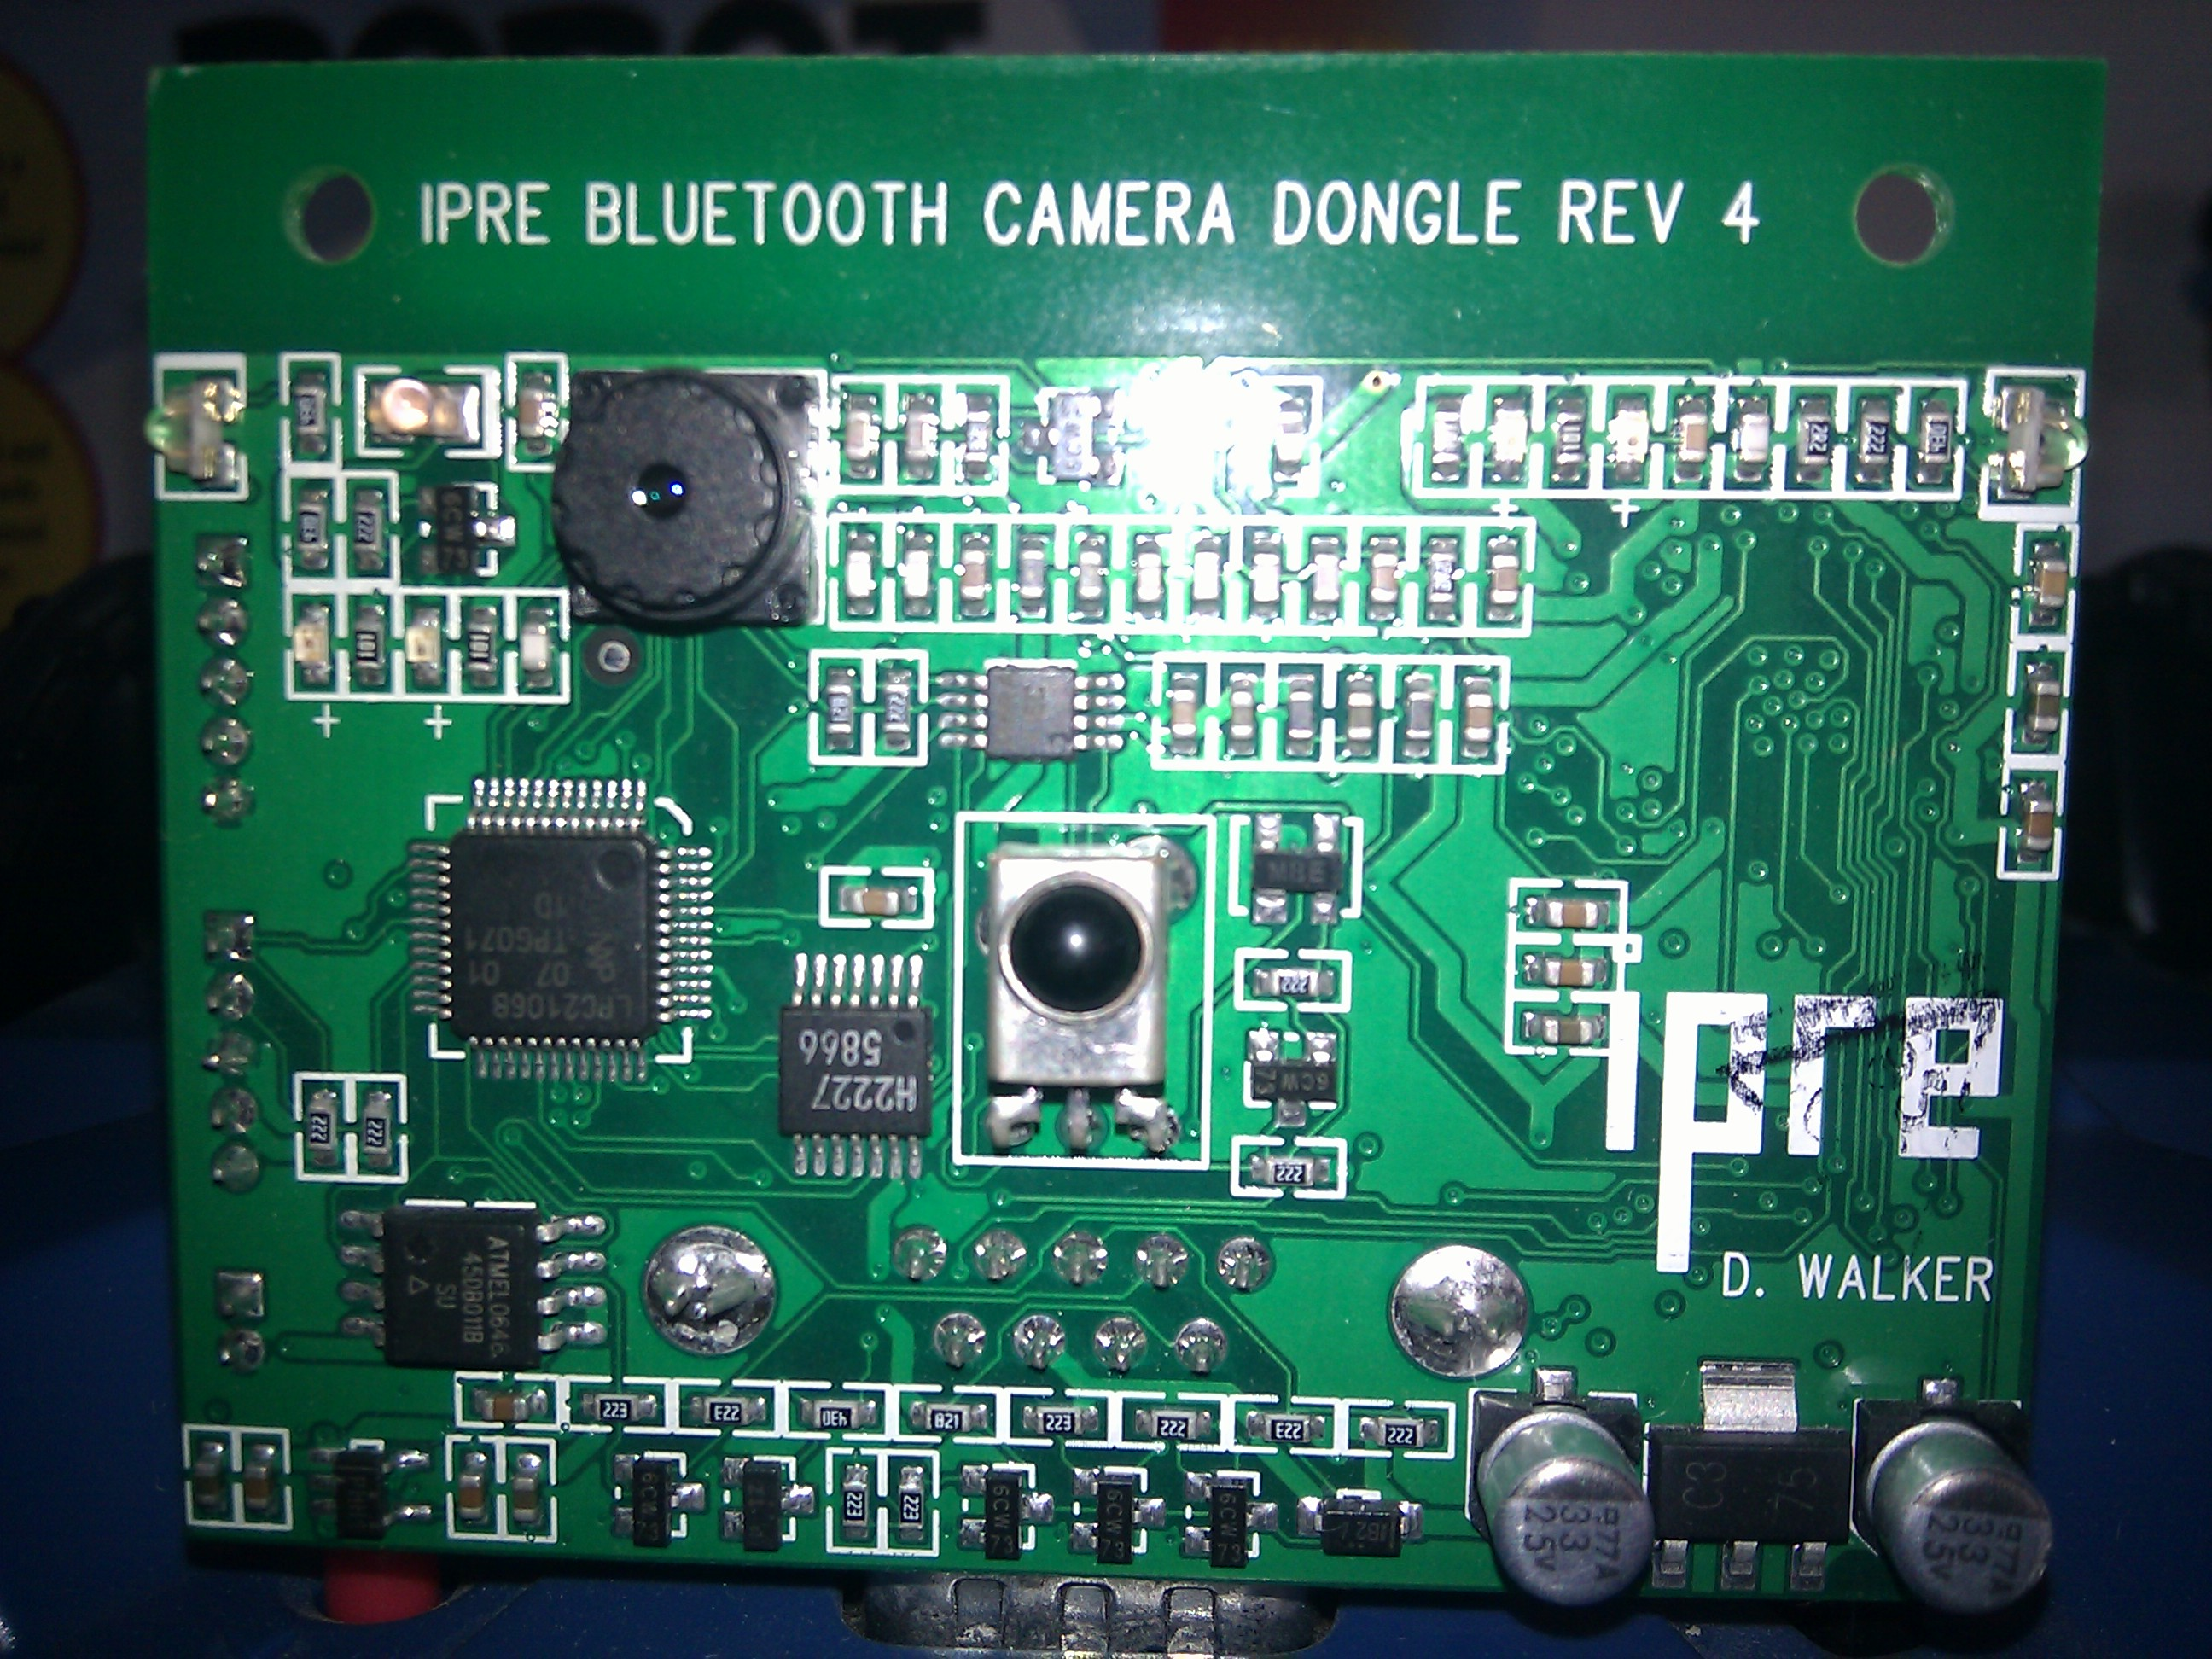
\includegraphics[width=\linewidth]{images/fluke}
        \end{figure}
    \end{minipage}
\end{frame}

\begin{frame}{Motivación}{Robots N6}
    \begin{minipage}[t]{0.7\linewidth}
        \begin{itemize}[<+->]
            \item Origen
            \item Biblioteca DuinoBot
            \item XBee
            \item Sensores
            \item Cómo los usamos
            \item Problemas:
                \begin{itemize}
                    \item Costos: XBee
                    \item Pilas
                \end{itemize}
        \end{itemize}
    \end{minipage}%
    \begin{minipage}[t]{0.3\linewidth}
        \begin{figure}
            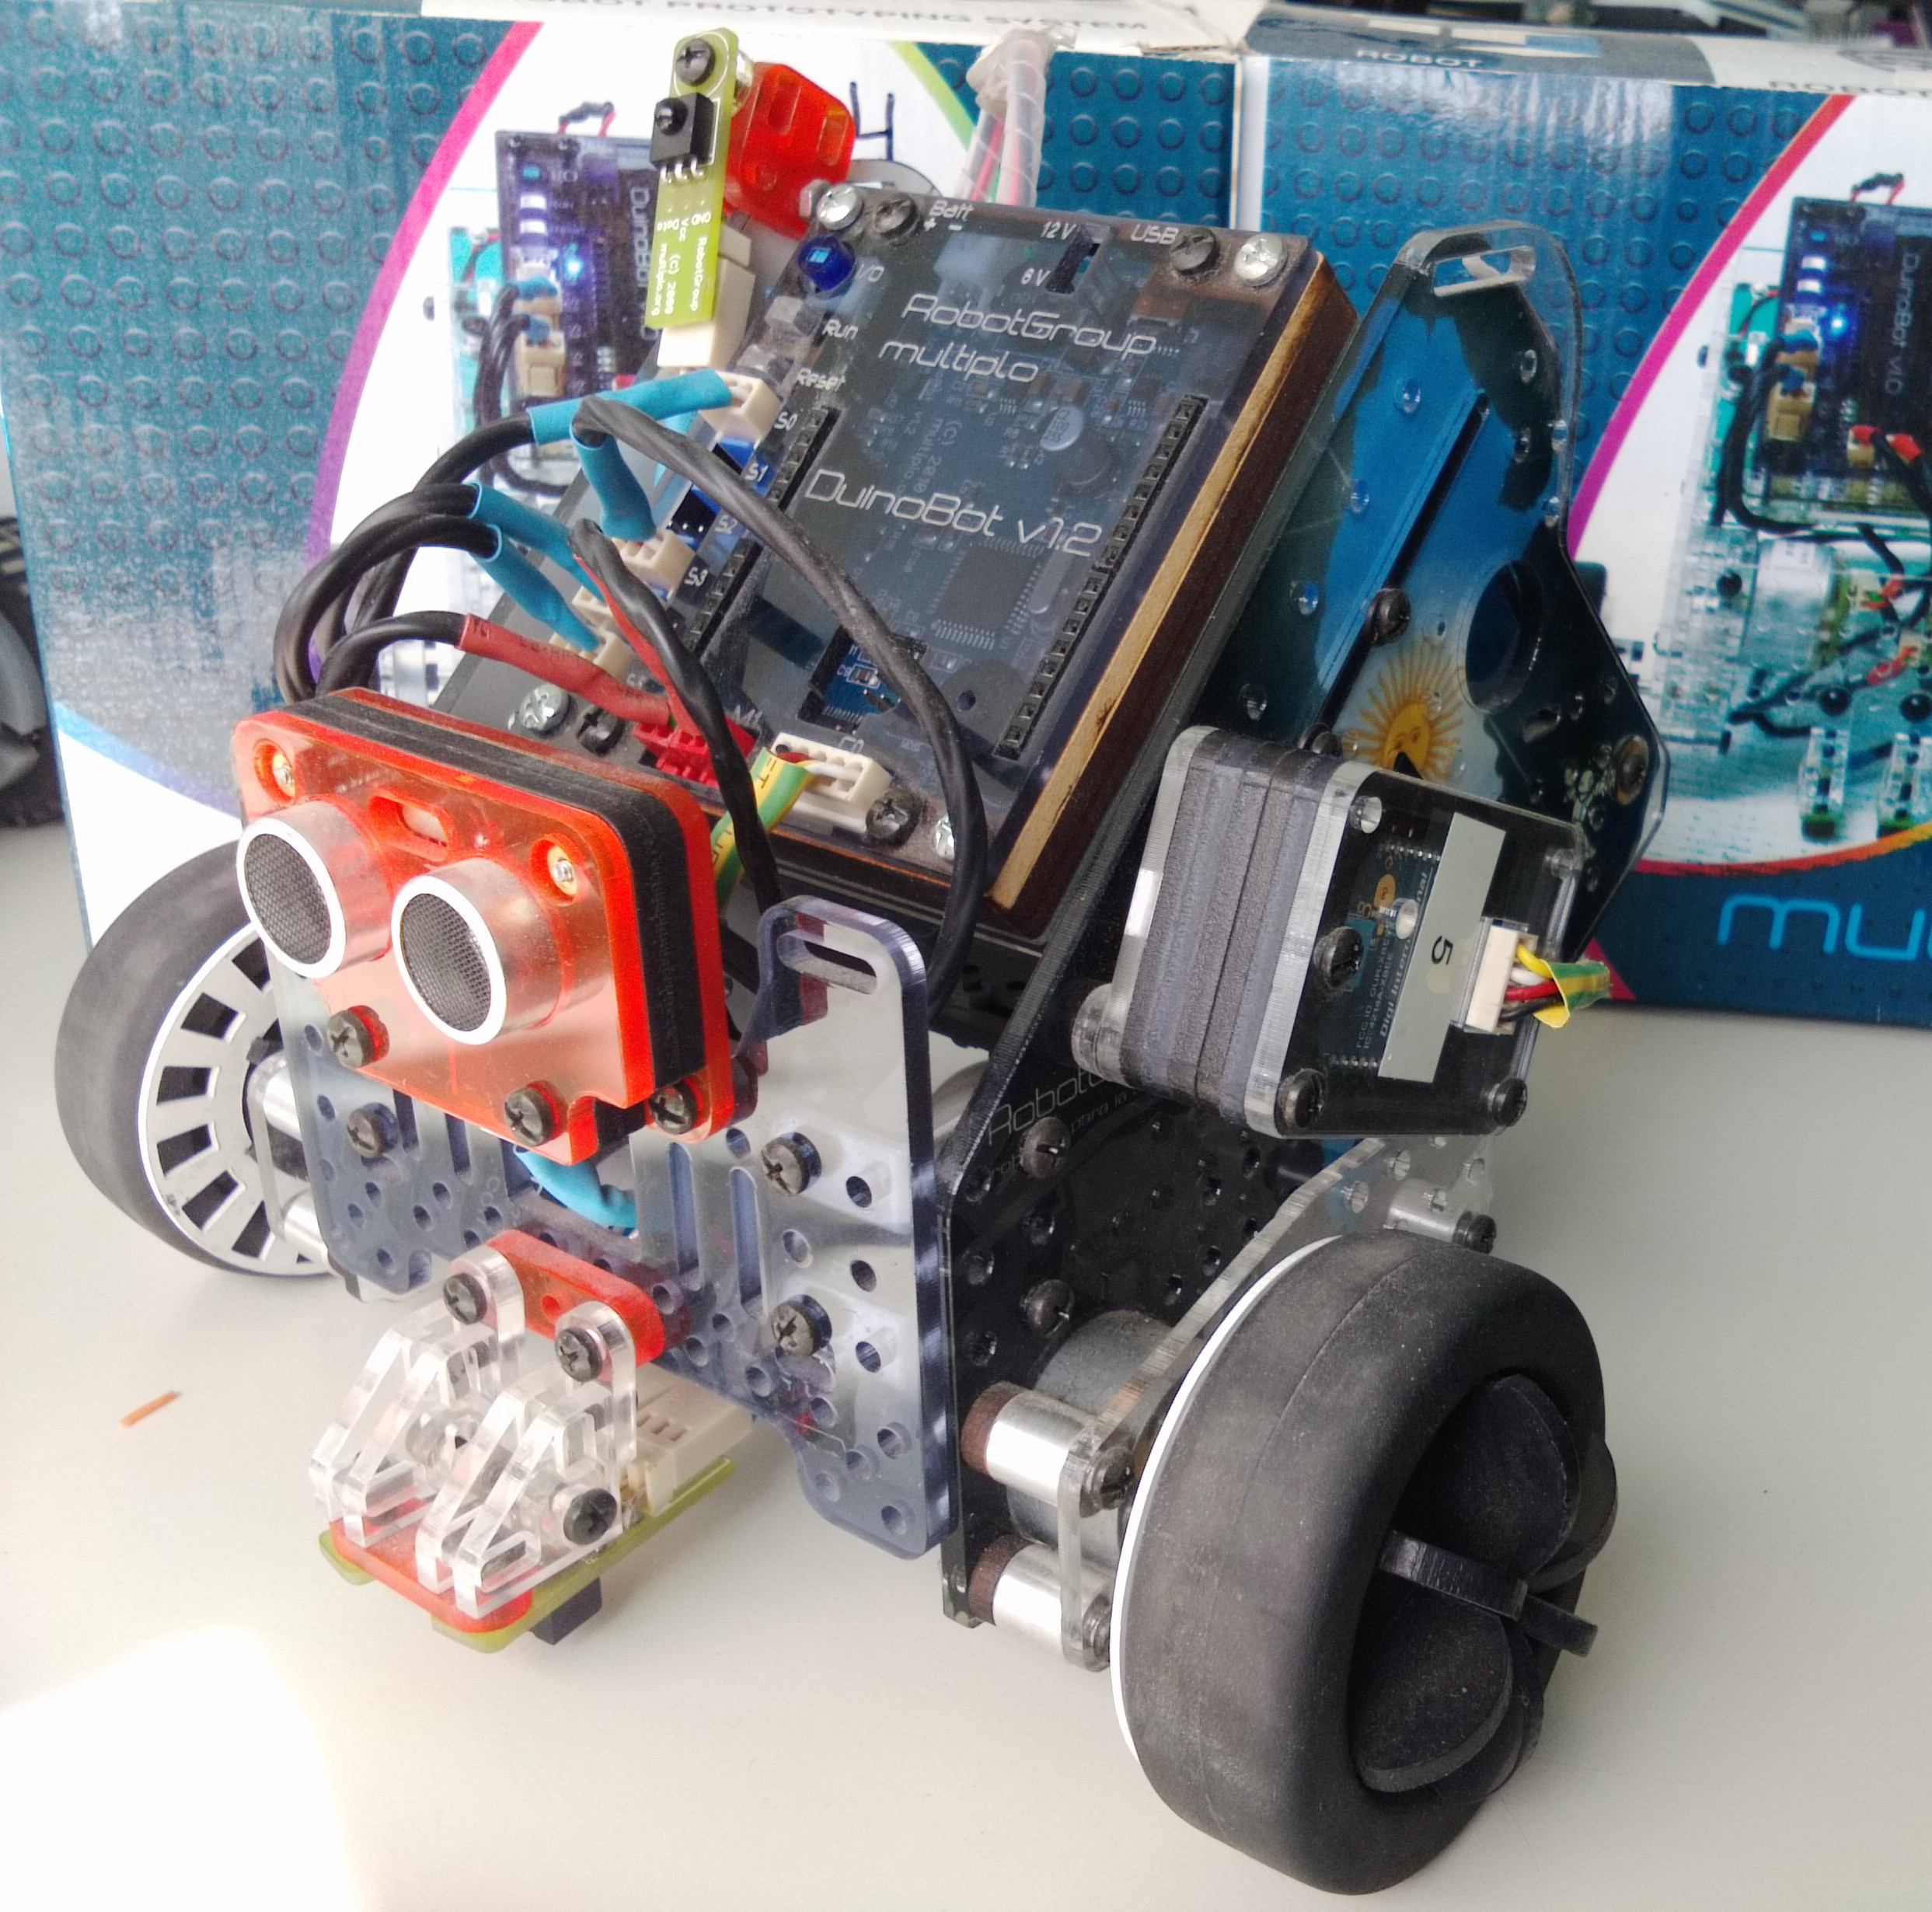
\includegraphics[width=\linewidth]{images/n6}
        \end{figure}
    \end{minipage}
\end{frame}

\begin{frame}{Motivación}{Trabajo final RemoteBot}
    \begin{minipage}{0.7\linewidth}
        \begin{itemize}[<+->]
            \item Laboratorio de software (2012)
            \item Aplicación Android en Java
            \begin{itemize}
                \item GUI
                \item Uso de sensores
                \item Uso de red
            \end{itemize}
            \item Incompatibilidad XBee
            \item Necesidad de un puente entre dispositivos:
            \begin{itemize}
                \item Python
                \item SimpleHTTPServer
                \item DuinoBot
            \end{itemize}
        \end{itemize}
    \end{minipage}%
    \begin{minipage}{0.3\linewidth}
        \begin{figure}
            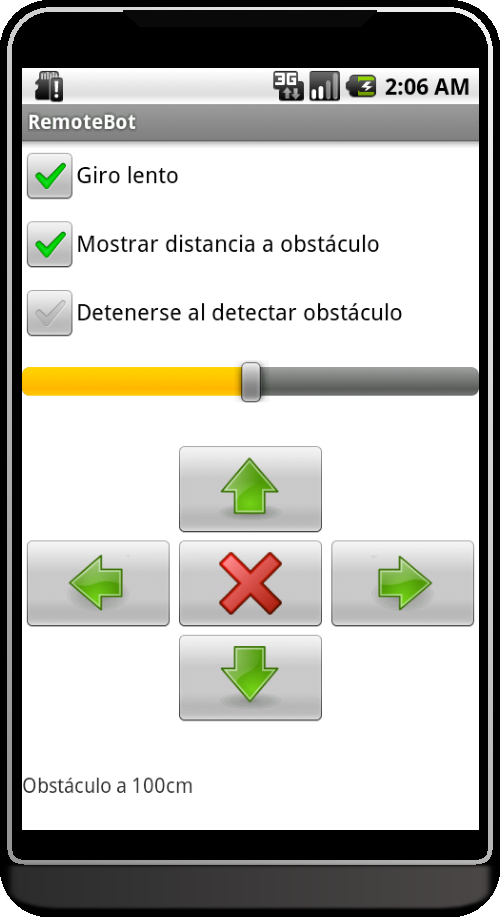
\includegraphics[width=\linewidth]{images/remotebot4android}
        \end{figure}
    \end{minipage}
\end{frame}

\begin{frame}{Motivación}{Experiencia posterior de la materia}
    \begin{minipage}{0.7\linewidth}
        \begin{itemize}[<+->]
            \item JDance: Otros alumnos intectuando con mi servidor
            \item Uso de toda la API JSON expuesta (métodos bloqueantes)
            \item Acceso concurrente
        \end{itemize}
    \end{minipage}%
    \begin{minipage}{0.3\linewidth}
        \begin{figure}
            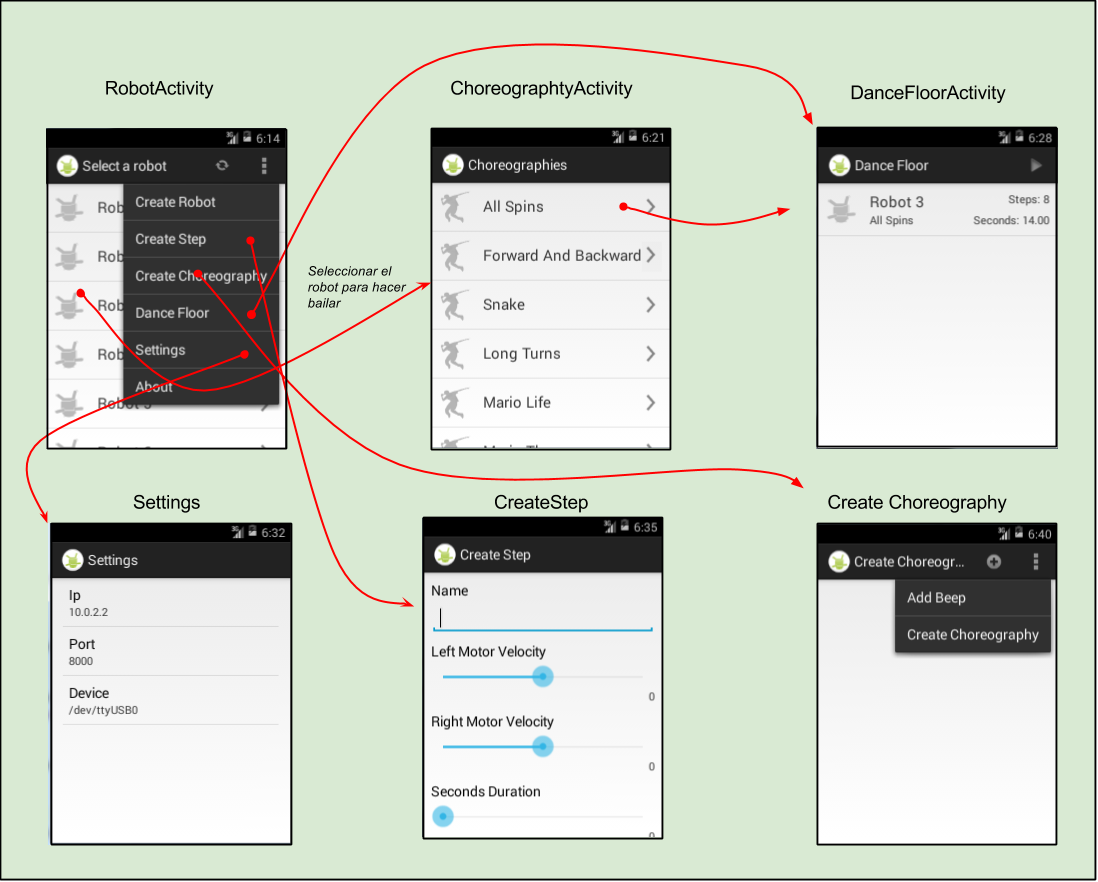
\includegraphics[width=\linewidth]{images/jdance}
            \caption{Una de las implementaciones de JDance}
        \vfill
        Fuente: \url{https://github.com/mclo/JDance}
        \end{figure}
    \end{minipage}
\end{frame}

\begin{frame}{Motivación}{Casos de uso posibles para una versión extendida}
    \begin{itemize}
        \item Acceso de los alumnos a los robots desde sus casas
        \item Compartir un solo XBee entre varios robots
        \item Permitir el uso de los robots en dispositivos móviles
    \end{itemize}
\end{frame}

\subsection{Control de robots a través de Internet}
\begin{frame}{Control de robots a través de Internet}{Posibilidades}
    \begin{itemize}[<+->]
        \item Experimentar sin miedo desde el hogar
        \item Afrontar los problemas de controlar un dispositivo real
        \item Acercar el proyecto a más gente
        \item Permitir el uso de otros lenguajes
        \item Otro enfoque posible: Ahorrar placas XBee
        \item Soportar otros robots con la misma biblioteca
    \end{itemize}
\end{frame}


\begin{frame}{Control de robots a través de Internet}{Opciones existentes de control de robots de forma remota}
    \begin{itemize}[<+->]
        \item Control de dispositivos:
        \begin{itemize}
            \item VCar
            \item Tele Toyland
        \end{itemize}
        \item APIs y plataformas:
        \begin{itemize}
            \item Educabot
            \item Gobot, Cylon y Artoo (The Hybrid Group)
            \item cppp-io
        \end{itemize}
    \end{itemize}
\end{frame}


\section{XRemoteBot}
\subsection{Diseño}

\begin{frame}{Diseño}{XRemoteBot}
    \begin{itemize}[<+->]
        \item Nombre XRemoteBot
        \item Inspirado en RemoteBot
        \item Reescrito
        \item Cliente-Servidor
    \end{itemize}
\end{frame}

\begin{frame}{Diseño}{Planteo de un servidor nuevo}
    \begin{itemize}[<+->]
        \item 2 modos de operación
        \item Variable \texttt{public\_server}:
            \begin{description}
                \item[\texttt{True}:]
                    \begin{itemize}
                        \item Requiere autenticación de los clientes
                        \item Marca los robots como ``reservados''
                        \item Pensado para ser usado a través de Internet
                    \end{itemize}
                \item[\texttt{False}]
                    \begin{itemize}
                        \item No requiere autenticación
                        \item Cualquier usuario puede usar cualquier robot
                        \item Pensado para ser usado en un aula
                    \end{itemize}
            \end{description}
    \end{itemize}
\end{frame}

\begin{frame}{Diseño}{Planteo de un nuevo procolo}
    \begin{itemize}[<+->]
        \item Transporte: Websockets
        \item Análisis de JSON, CBOR y BSON:
        \begin{itemize}
            \item Velocidad
            \item Bytes por mensaje
            \item Sin diferencias significativas en Python
            \item Diferencias en la velocidad en Javascript
            \item Se prioriza el soporte para el browser: JSON
        \end{itemize}
    \end{itemize}
\end{frame}

\begin{frame}{Diseño}{API JSON}
    \begin{itemize}[<+->]
        \item Protocolo simple y extensible
        \item Mensajes del cliente:
        \begin{itemize}
            \item \texttt{entity}
            \item \texttt{method}
            \item \texttt{args}
        \end{itemize}
        \item Respuestas del servidor:
        \begin{itemize}
            \item \texttt{response}
            \item \texttt{value}
            \item \texttt{message}
        \end{itemize}
        \item \texttt{msg\_id}: Opcional
    \end{itemize}
\end{frame}


\begin{frame}{Diseño}{Características comunes entre el N6 y el Scribbler}
    \begin{itemize}[<+->]
        \item Posibilidades de movimiento
        \item Sensores principales
        \item Lenguaje de las bibliotecas
        \item Interfaz de programación similar
        \item Módulos de Python específicos para cada uno
        \item Posibilidad de unificar las APIs
    \end{itemize}
\end{frame}

\subsection{Implementación}
\begin{frame}{Implementación}{Características de XRemoteBot}
    \begin{itemize}[<+->]
        \item Soporte de robots Scribblers y Multiplo con la misma API
        \item Sistema de reservas de los robots
        \item Servidor con soporte de concurrencia
        \item Extensible a otros robots (u otros dispositivos)
        \item Protocolo accesible desde Javascript
        \item Selección de tecnologías que habilita el uso de Javascript
            desde un navegador
        \item Clientes simples en general
    \end{itemize}
\end{frame}

\begin{frame}{Instalación actual}
    \begin{minipage}{0.5\linewidth}
        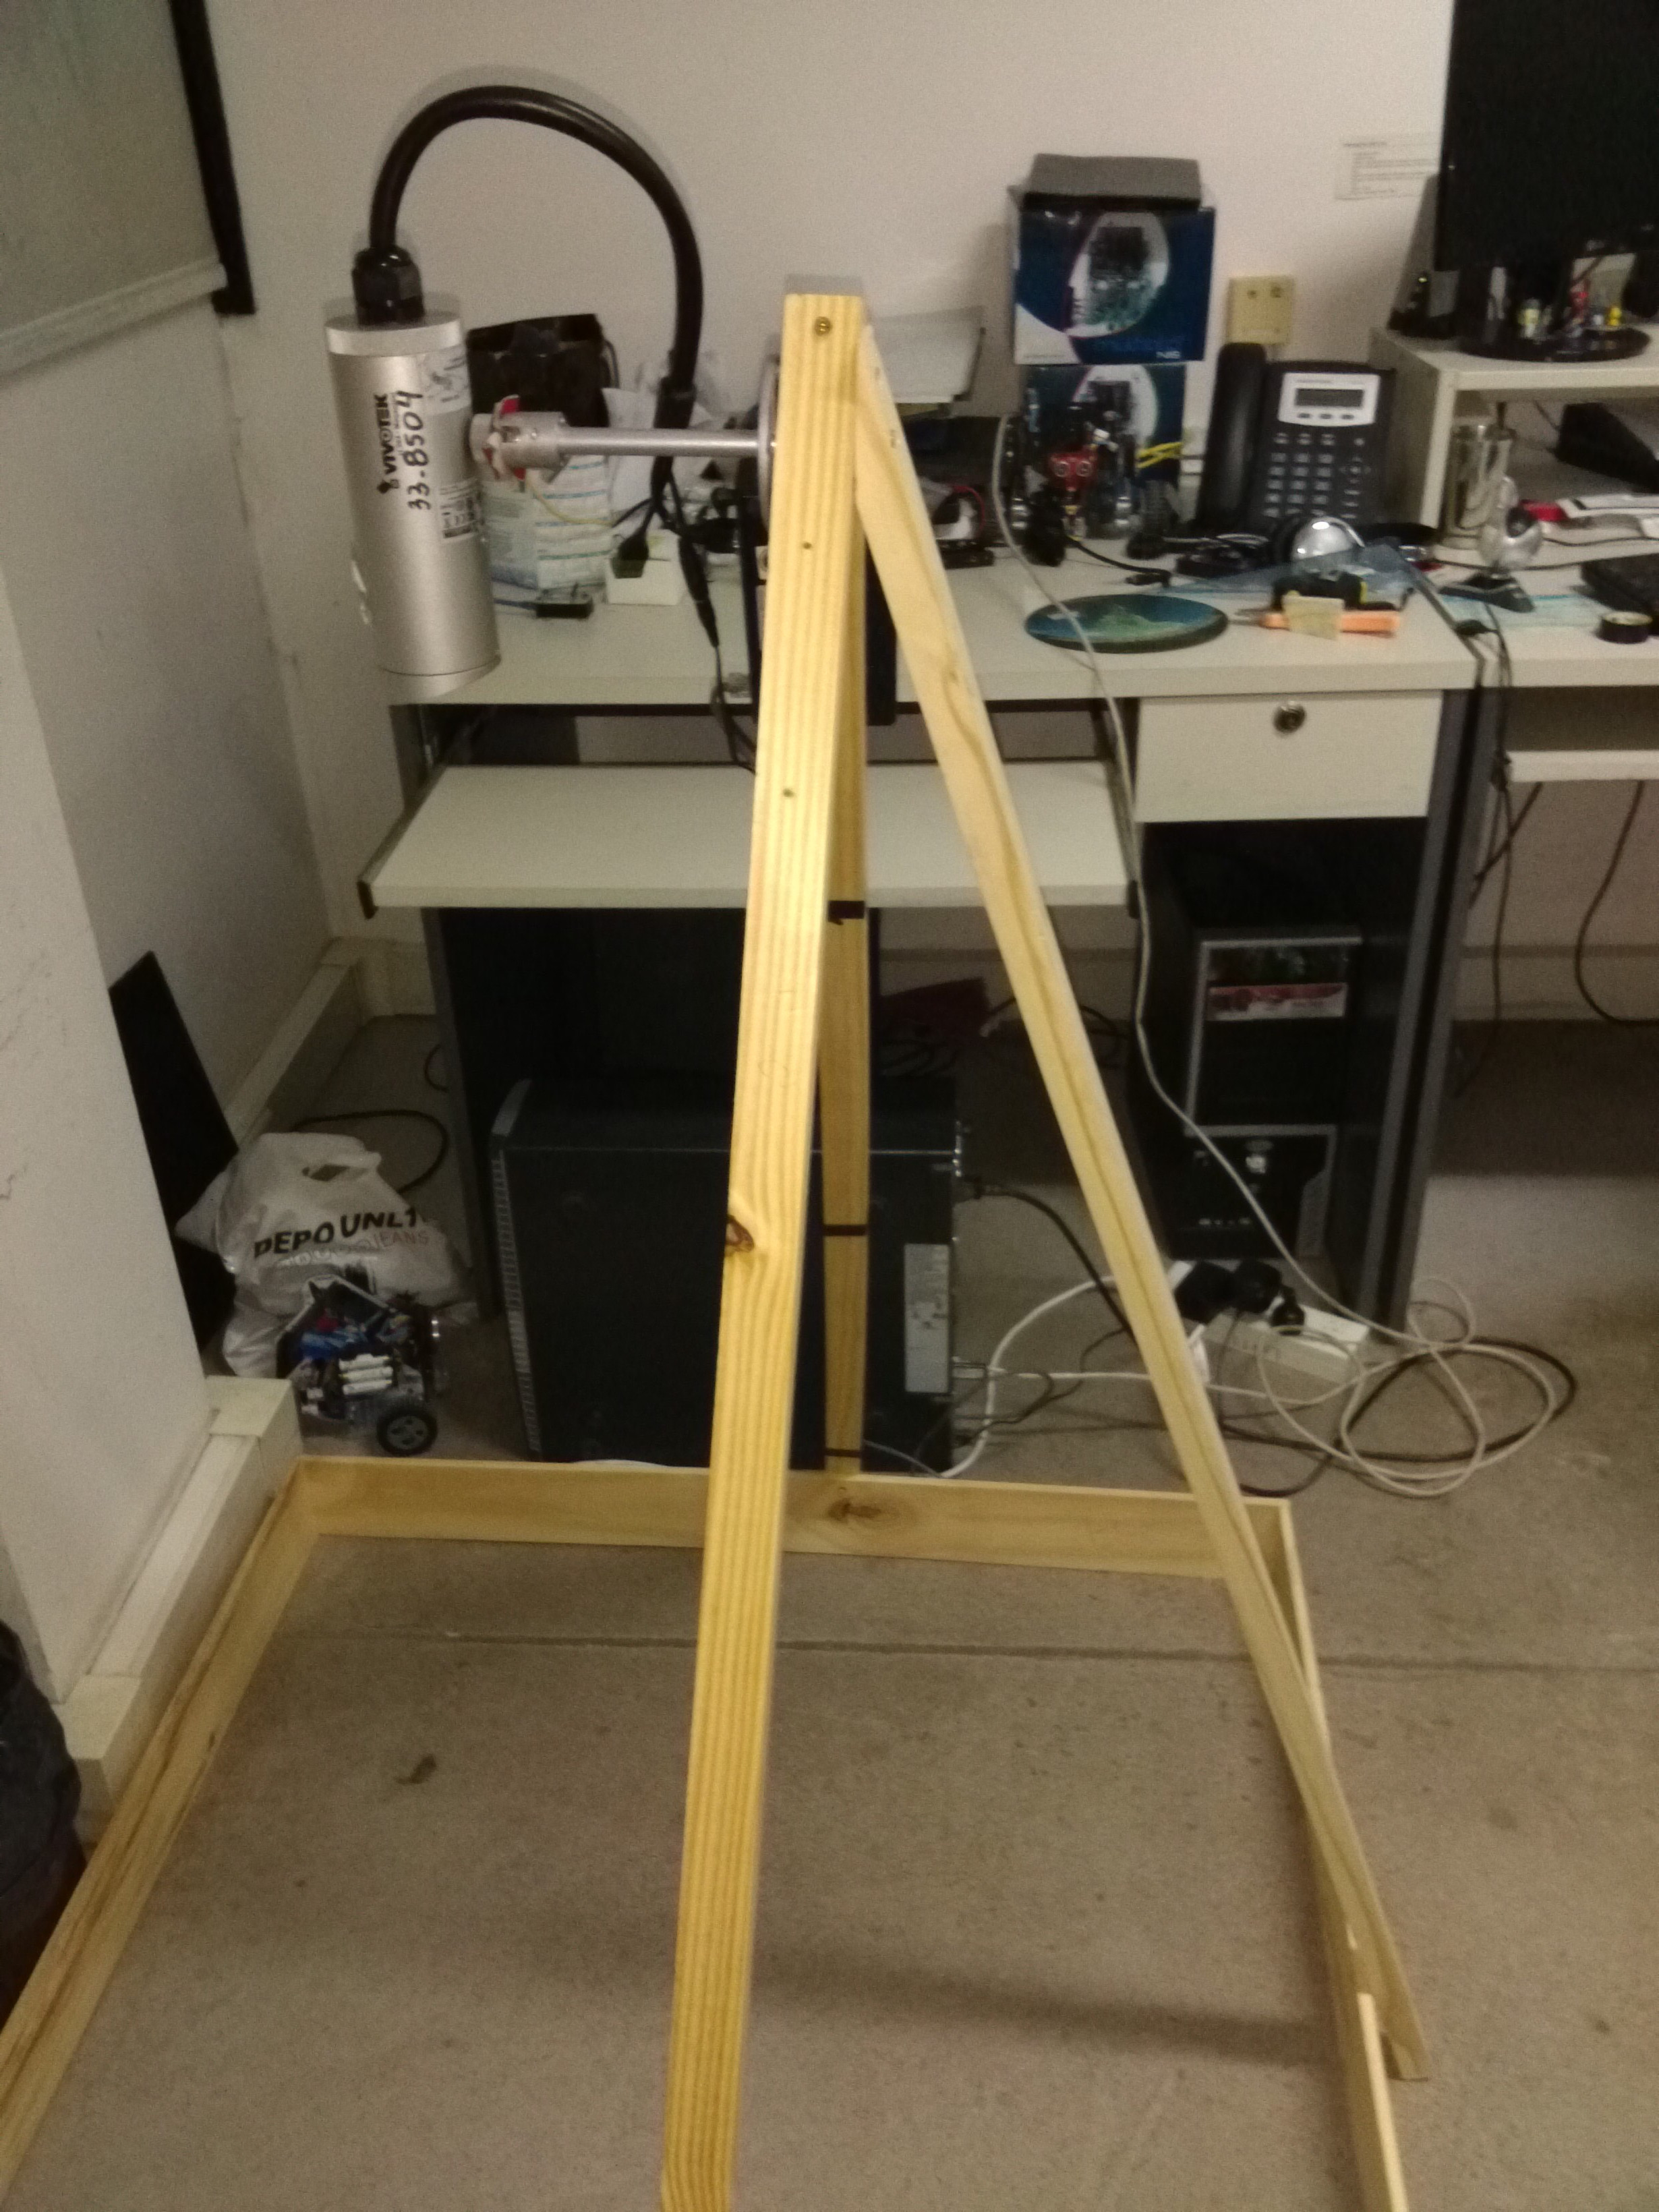
\includegraphics[width=\linewidth]{images/inst1}
    \end{minipage}%
    \begin{minipage}{0.5\linewidth}
        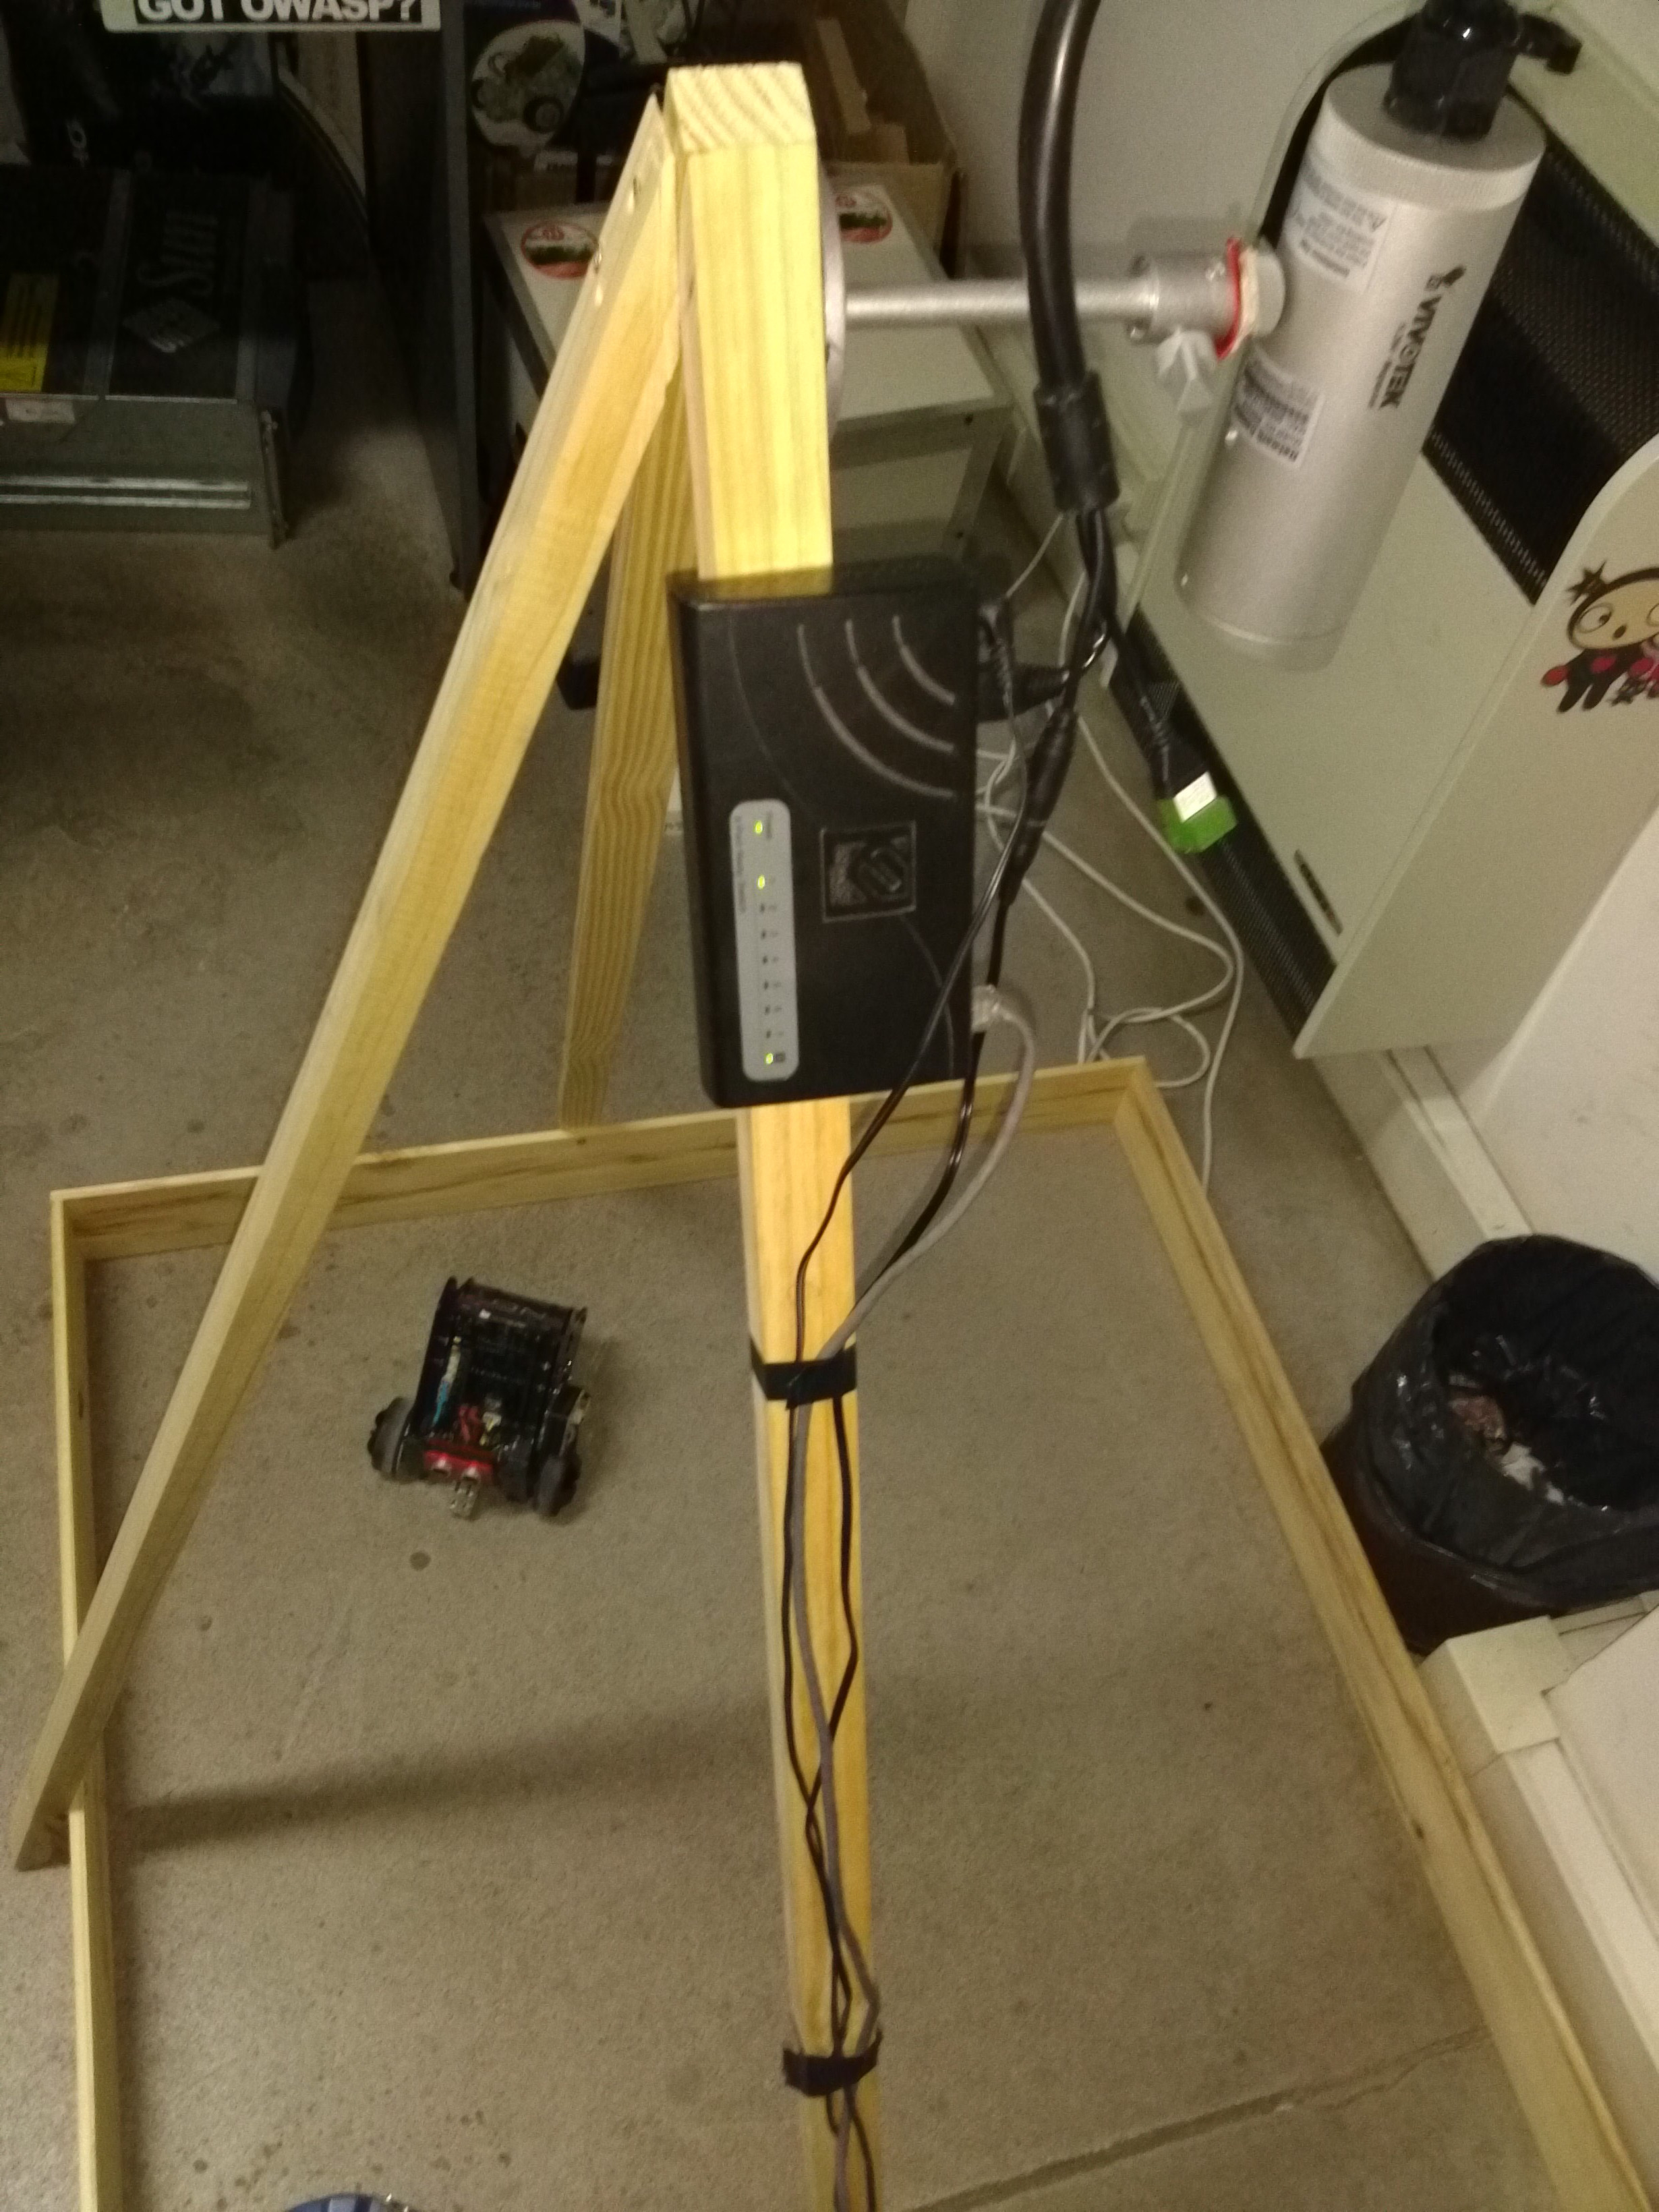
\includegraphics[width=\linewidth]{images/inst2}
    \end{minipage}
\end{frame}

\begin{frame}{Implementación}{Clientes de XRemoteBot}
    \begin{itemize}[<+->]
        \item Python
        \item Ruby
        \item Javascript
        \begin{itemize}
            \item API de WebSockets
            \item Promises
        \end{itemize}
        \item Interfaz Web (\href{run:ejemplos/interfaz.mp4}{video})
    \end{itemize}
\end{frame}

\section{Ejemplos}
\subsection{Movimientos básicos}
\begin{frame}{Ejemplos}{Movimientos básicos}
    \begin{minipage}{0.45\linewidth}
        \lstinputlisting[caption=Python,language=Python]{ejemplos/cuadrado.py}
    \end{minipage}\hspace{0.1\linewidth}%
    \begin{minipage}{0.45\linewidth}
        \lstinputlisting[caption=Ruby,language=Ruby]{ejemplos/cuadrado.rb}
    \end{minipage}
\end{frame}

\begin{frame}[fragile]{Ejemplos}{Movimientos básicos}
    \lstinputlisting[caption=Javascript,language=C]{ejemplos/cuadrado.js}
\end{frame}

\subsection{Esquivar obstáculos}
\begin{frame}{Ejemplos}{Esquivar obstáculos}
    \begin{minipage}{0.45\linewidth}
        \lstinputlisting[caption=Python,language=Python,linerange=1-18]{ejemplos/esquivar.py}
    \end{minipage}\hspace{0.1\linewidth}%
    \begin{minipage}{0.45\linewidth}
        \lstinputlisting[caption=Ruby,language=Ruby]{ejemplos/esquivar.rb}
    \end{minipage}
\end{frame}

\begin{frame}[fragile]{Ejemplos}{Esquivar obstáculos}
    \lstinputlisting[caption=Javascript,language=C]{ejemplos/esquivar.js}
\end{frame}

\subsection{Valores de los sensores en la vista Web}
\begin{frame}[fragile]{Ejemplos}{Sensores}
    \lstinputlisting[caption=Javascript,language=C,linerange=1-18]{ejemplos/senses.js}
    (\href{run:ejemplos/senses.mp4}{video})
\end{frame}

\subsection{Control remoto}
\begin{frame}[fragile]{Ejemplos}{Control remoto con botones}
    \lstinputlisting[caption=Javascript,language=C]{ejemplos/botones.js}
    (\href{run:ejemplos/botones.mp4}{video})
\end{frame}

\section{Trabajos futuros}
\begin{frame}{Trabajos futuros}
    \begin{itemize}[<+->]
        \item Brython, Opal, Blockly
        \item Integración con moodle
        \item Almacenamiento de programas con la API LocalStorage o en el servidor
        \item Streaming: UStream, Youtube, etc...
    \end{itemize}
\end{frame}



            %\begin{itemize}
            %    \item Fundación YPF
            %    \item Dirección de Escuelas Técnicas de la Provincia de
            %        Buenos Aires
            %\end{itemize}
%
% Diferencias
% XRemoteBot: 726 LOCs Python
% RemoteBot: 156 LOCs Python
% * Se excluyeron lineas en blanco, comentarios, definiciones de funciones y
% definiciones de clases.

\begin{frame}{Links}
    \begin{description}
        \item[Servidor:]
            \href{https://github.com/fernandolopez/xremotebot.git}
            {https://github.com/fernandolopez/xremotebot.git}
        \item[Clientes:]
            \href{https://github.com/fernandolopez/xremotebot-clients.git}
            {https://github.com/fernandolopez/xremotebot-clients.git}
    \end{description}
\end{frame}

\begin{frame}
    \centering
    
\includegraphics[width=0.2\linewidth]{images/cc-by}

    Esta obra está licenciada bajo la Licencia Creative Commons Atribución
    4.0 Internacional. Para ver una copia de esta licencia, visita
    \url{http://creativecommons.org/licenses/by/4.0/}.
\end{frame}

\end{document}
